\documentclass[12pt,info]{asg}
% General info for the asg.cls file to load
\Instructor{Anna Koop}
\Campus{University of Alberta, Augustana}
\Email{akoop@ualberta.ca}
\Office{Heather Brae 1-31}
\Class{AUCSC 370}
\ClassTitle{Programming Languages}
\Term{Fall 2016}
\Department{Department of Science}


\AsgNum{Final}
\AsgTitle{Assigning Preferences}
\Due{11:55pm, Dec 14, 2016}
\Total{30}

\title{Assigning Ranked Preferences}

\begin{document}

\maketitle
\section*{Objectives}
\begin{itemize}
\item To demonstrate your ability to think in different programming styles.
\item To examine the strengths and weaknesses of Scheme, Prolog, and C in a real-world problem.
\item To experience and reflect on how different programming paradigms approach the same problem.
\end{itemize}

\section*{Problem Specification}
Beginning in 2017, First-year students to Augustana will be enrolled in a "First Year Seminar", a 3-week discussion-based research course designed to introduce new students to university-level scholarship. A wide variety of seminars have been proposed, but space is limited.

New students will be asked to pick their top three choices from the available classes. Then comes the difficult task of actually assigning students to classes in a way that respects physical constraints (no more than 25 per class, and only one offering of each class) while optimizing happiness (as much as possible we want people to get their top choices).

\section*{Program Specification}
Computers to the rescue. You will write three versions of the program for doing this: one in C, one in Scheme, and one in Prolog. We will use a simple scoring mechanism for evaluating the quality of the match. The match will give every student a disappointment number: 0 if they got into their first choice, 1 for second, 2 for third, and 5 for being assigned one they did not choose. The total score is the sum over all students. 

This means 0 is perfection---everyone got into their first choice. Highly unlikely. Optimizing the assignment is a difficult problem in general so you {\em do not} have to find the single best solution for the given data. The score is simply to evaluate the matches programs find.

\subsection*{Input}

The data structures and control flow are completely up to you and, of course, will be different for each language. The input you have to work with will be in two text files. First gives the full list of course identifiers and possible associated information, eg:
\begin{lstlisting}[language=Lisp]
	FYS111, Drugs
	FYS112, Murder!
	FYS113, How to be a Doctor
	FYS114, Machine Apocalypse
	...
\end{lstlisting}
The second gives a list of students and their top three preferences.
\begin{lstlisting}[language=Lisp]
	1011111, FYS114, FYS111, FYS122
	1011112, FYS111, FYS122, FYS199
	...
\end{lstlisting}

\subsection*{Output}
Your program will read these files and display a table assigning students to each class:
\begin{lstlisting}[language=Lisp]
	FYS111, 1011111, 1011113, 1011114, 1022222...
	FYS112, 1111112, 1011112, 1011115, 1022223...
	...
\end{lstlisting}

A proper solution must satisfy the following characteristics:
\begin{itemize}
\item All students are assigned to one and only one class.
\item All student identifiers are valid.
\item No class has more than 25 students.
\item All class identifiers are valid.
\item No class has less than 10 students\footnote{This restriction may be changed after consultation with stakeholders}.
\item The matching score passes a minimum bar\footnote{TBD and posted in eClass}.
\end{itemize}

\section*{Report}

In addition to the three program files, you will submit a (no more than 3-page) report. Your report should examine the strengths and weaknesses of each particular language {\em and} overall language paradigm for the task. 

\subsection*{Introduction}
Start with a brief, high-level description of your approach in each language. This includes what data structures and control flow you used or took into account.

\subsection*{Body}
The focus of the report is on comparing and contrasting your use of the languages for this problem. What was different about the algorithm or program structure in each? What was similar? You may include personal details (eg. difficulty, time) as well as technical information (eg. efficiency, readability, etc).

\subsection*{Conclusion}
Conclude with a recommendation for the 'best' language for this problem. Be sure to support your recommendation appropriately.

This is a formal report and you will be graded on clarity, structure, and grammar as well as the critical thought and  knowledge demonstrated in the report.


\section*{Grading}

Each program is marked out of 50 and worth 5\% of your final grade. The report is marked out of 60 and is worth 15\% of your final grade.

\subsection*{Program Code}
Code compiles (on park) according to instructions and/or runs in the (web-based) interpreters without error. /15

The results are displayed in a readable format according to the specification. The results are valid according to the given criteria. /10

The code is well documented and readable. /10

The solution approach is appropriate for the given language. /10

The code demonstrates skill in the language constructs and idioms. /5

\subsection*{Report}
The report is complete. It provides overview, detail, and comparison between all the languages as described in the specification. /10

The report is well organized, grammatically correct, and clear. /10

The report is factually correct and accurately explains relevant concepts. /20

The report demonstrates thoughtfulness and insight in relation to both project and course concepts. /20


%%%%%%%%%%%%
%\begin{figure}[bt]
%\label{fig:adder}
%\centering
%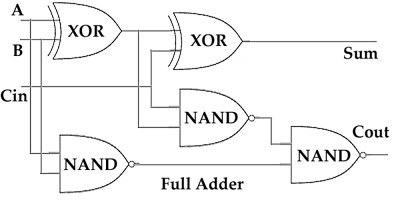
\includegraphics[width=.6\textwidth]{full_adder.png}
%\caption{A (claimed) full-adder circuit}
%\end{figure}

%\newcounter{rubricCat}
%\newcounter{rubricVal}
%\newlength{\colwidth}

%\newenvironment{rubric}[1]{%
%	\setcounter{GradeCategories}{#1}
%	\begin{landscape}
%	\begin{table}[t]
%	\begin{center}
%	\begin{tabulary}{.8\textwidth}{ l | *{5}{c}}
%	 & Excellent & Good & Acceptable & Needs Work & Absentee \\
%	 \end{tabulary}
%	 \end{center}
%	 \end{table}
%	\end{landscape}
%} % rubric environment

\end{document}
